\documentclass[spanish,12pt,a4paper,titlepage]{report}
\usepackage[utf8]{inputenc}
\usepackage{graphicx}
\usepackage{subfig}
\usepackage{float}
\usepackage{wrapfig}
\usepackage{multirow}
\usepackage{caption}
\usepackage[spanish]{babel}
\usepackage[dvips]{hyperref}
\usepackage{amssymb}
\usepackage{listings}
\usepackage{epsfig}
\usepackage{amsmath}
\usepackage{array}
\usepackage[table]{xcolor}
\usepackage{multirow}
%\usepackage[Sonny]{fncychap}
\usepackage[Lenny]{fncychap}
%\usepackage[Glenn]{fncychap}
%\usepackage[Conny]{fncychap}
%\usepackage[Rejne]{fncychap}
%\usepackage[Bjarne]{fncychap}
%\usepackage[Bjornstrup]{fncychap}

%\usepackage{subfiles}
%\usepackage{framed}

\setlength{\topmargin}{-1.5cm}
\setlength{\textheight}{25cm}
\setlength{\oddsidemargin}{0.3cm} 
\setlength{\textwidth}{15cm}
\setlength{\columnsep}{0cm}

\begin{document}

\chapter{GPS - Test 2}
\label{chap-gps-test-2}

\section{Objetivos}
%\ref{} agregar refs
%TODO esta ref es trucha! cambiar por la posta!!
\label{chap-gps-test-1}

En el capítulo anterior se comenzó a analizar la performance del GPS. Se intentó reconstruir un polígono, y se analizó el error al estimar la posición de un punto fijo. En este capítulo se continúa dicho análisis, repitiendo el procedimiento, pero con un polígono más grande, y tiempo más largos para la estimación de la posición de un punto fijo.

\section{Materiales}

\begin{itemize}
\item GPS.
\item Laptop.
\item Trípode (de fotografía.
\item Cinta métrica, pintura y cuerda.
\end{itemize}

\newpage
\section{Procedimiento}
\label{sec:gps2-procedimiento}

En esta prueba se trata de obtener el error del GPS en el plano paralelo a la tierra, es decir, el error en latitud y longitud.

El experimento que se diseñó consiste en marcar un rectángulo sobre el suelo (pasto), utilizando 6 puntos, con la siguiente disposición:

\begin{quote}
\begin{quote}
\begin{quote}
\begin{verbatim}

      Árbol              
 Árbol               Árbol
           Gente_q_me_va_a_afanar
      Árbol
 -- < -- < -- < -- < -- < -- < -- <
    calle que sube de la rambla
 -- > -- > -- > -- > -- > -- > -- > 
 3                2                1
 x ---- ---- ---- x ---- ---- ---- x
 |                                 |
 |                                 |
 
 |                                 |
 |                                 |
 x ---- ---- ---- x ---- ---- ---- x
 6                5                4

     Estacionamiento de la fac

 Orientación del GPS:

                    led
                     ^
                     |
                     |
                    usb

\end{verbatim}
\end{quote}
\end{quote}
\end{quote}

A diferencia del experimento de la sección \ref{chap-gps-test-1}, aqui todas líneas punteadas son de 6m de largo, en lugar de 1m. Resulta en un rectángulo de 6m por 12m.

Los pasos a seguir son los siguientes:

\begin{enumerate}
\item Construir el rectángulo sobre un superficie plana.
  \begin{itemize}
  \item Se utilizó pintura para marcar los vértices del triángulo.
  \item Para trazar uno de los lados de 12 metros (puntos 1,2 y 3), se fijó una cuerda de 12 metros (con el punto medio marcado) a un punto, y se extendió (sin estirarla). El principio (\verb+1+) y el final (\verb+3+) de la cuerda son vértices del polígono, y el punto medio (\verb+2+) es otro de los puntos de interés.
  \item Para construir perpendículares se utilizó una cuerda de 6m, y otra de 8.5m\footnote{Pitágoras: $8.5 \approx \sqrt{6^2 + 6^2} = 8.4852...$}. Uno de los extremos de la cuerda de 6 metros se fijó al \verb+1+, y uno de los extremos de la cuerda de 8.5m se fijó a \verb+2+. El punto donde ambas se intersectan corresponde a \verb+4+. Un procedimiento similar se siguió para determinar la ubicación de \verb+5+ y \verb+6+.
  \end{itemize}
\item Medir, con un metro, las distancias entre todos los puntos.
\item Utilizar mínimos cuadrados para minimizar el error entre las distancias esperadas, y las experimentales. Esto puede llevar a trabajar con un polígono que \textbf{no} sea un rectángulo, pero el error será menor que el que resultaría de usar los valores teóricos.
\item Fijar la altura y la orientación del GPS, y tomar medidas en cada uno de los puntos \verb+[1,2,3,4,5,6]+.
\item Tomar un punto como origen, y comparar la figura que resulta de los datos provenientes del GPS con las medidas tomadas con el metro.
\end{enumerate}

En la figura \ref{fig:tripode_con_plomada.jpg} se observa el trípode que sostiene al GPS. El objetivo era tener el GPS a una altura fija, y separado del piso. Al nivel del piso los rebotes degradan seriamente la performance del GPS. La cuerda que marca el lado del polígono, junto con las patas del trípode, se utilizaron para fijar la orientación del GPS durante el experimento.

\begin{figure} [h!]
  \centering
  \subfloat[Trípode de fotografía, con el GPS atado en lugar de la cámara..]{\label{fig:tripode_con_plomada.jpg}
  		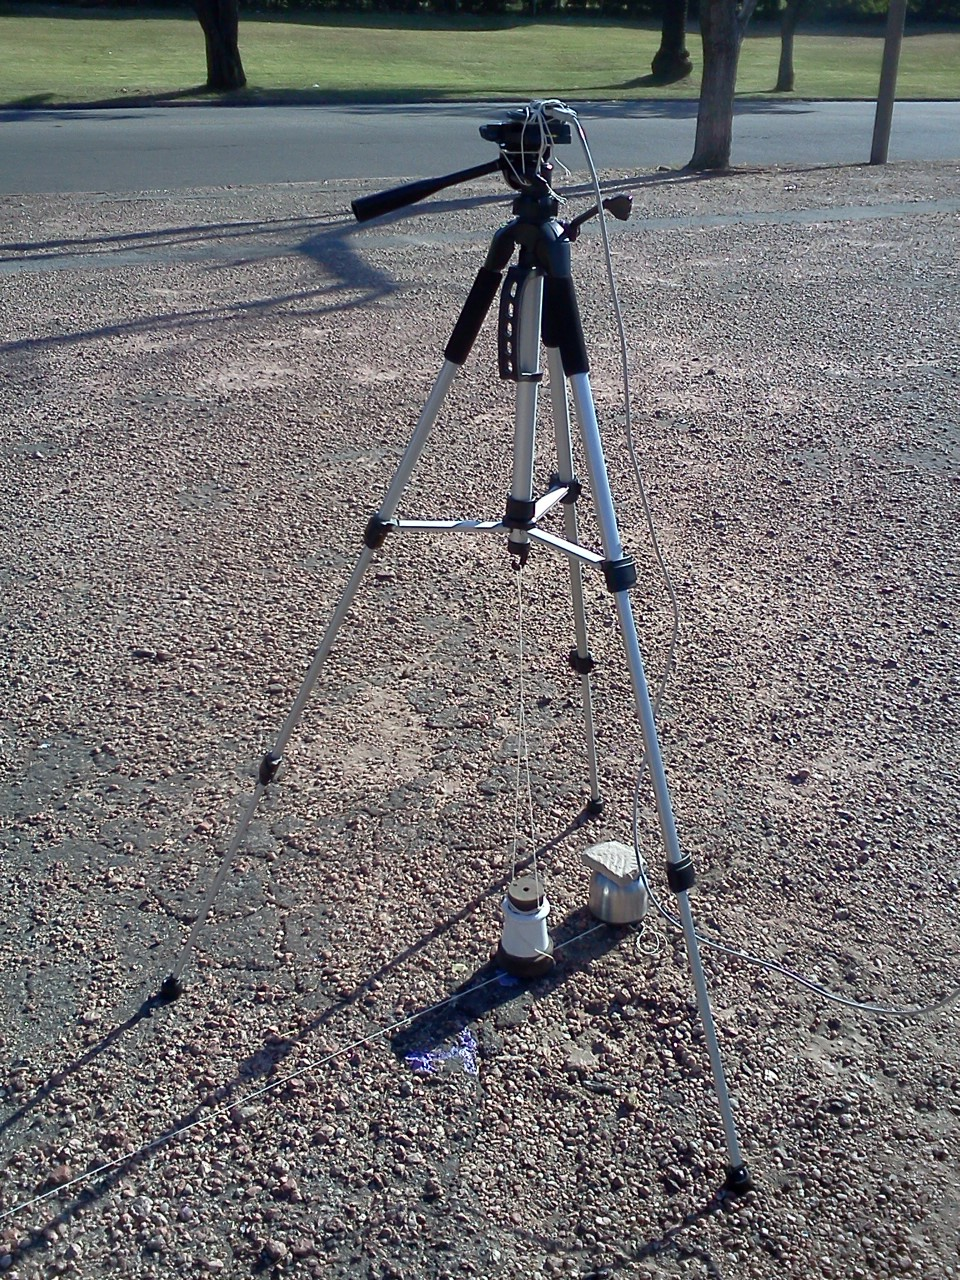
\includegraphics[width=0.45\textwidth]{./img/tripode_con_plomada.jpg}}
  \subfloat[GPS amarrado al trípode.]{\label{fig:vista_usb.jpg}
  		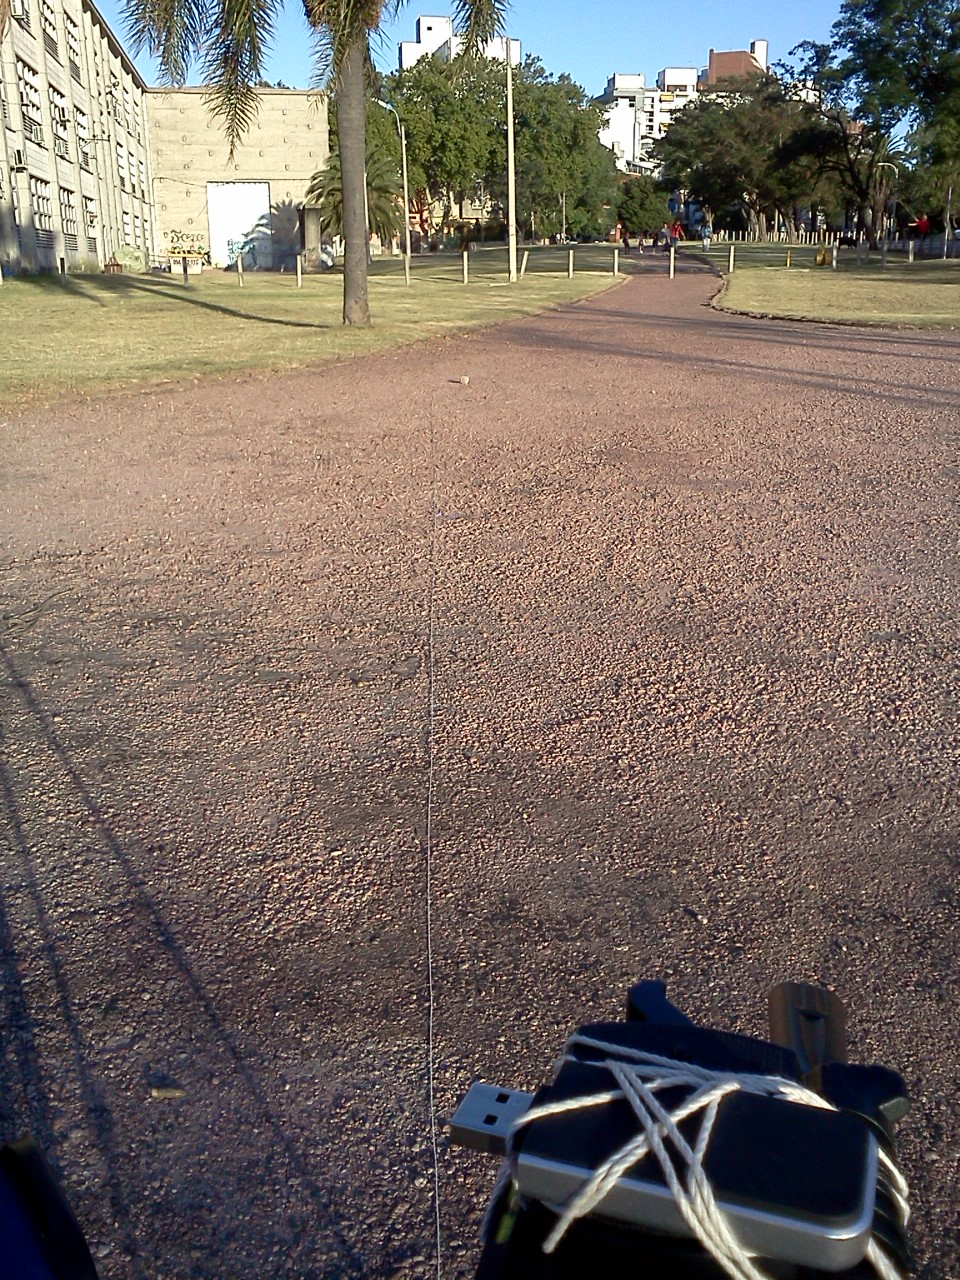
\includegraphics[width=0.45\textwidth]{./img/vista_usb.jpg}}
  \caption{GPS + Atril}
  \label{fig:rebotes}
\end{figure}

\newpage
\subsection{Verificación del polígono}
\label{sec:verificacion-del-poligono}

Una vez construído el polígono, es de interés medir todas las diagonales (con la cinta métrica) por dos motivos:
\begin{itemize}
\item Verificar que no se cometieron errores.
\item Hacer mínimos cuadrados con las medidas, de manera de obtener un polígono, que no tiene porqué ser (y en general no será) un rectángulo, sino algo similar a un rectángulo, más ajustado a la realidad.
\end{itemize}

Las medidas tomadas se resumen en la tabla \ref{tab:diagonales-poligono}, donde \verb+D12+ representa la medida de la recta que une el punto \verb+1+ con el punto \verb+2+, en cm.

\begin{table}[H]
\begin{center}
\begin{tabular}{|c|c|c|c|c|c|c|c|c|c|c|c|c|}
\hline
D12 & D14 & D15 & D16 & D23 & D24 & D25 & D26 & D34 & D35 & D36 & D45 & D56 \\
\hline
603 & 606 & 855 & 1345 & 603 & 853 & 608 & 853 & 1344 & 850 & 602 & 602 & 603 \\
\hline
\end{tabular}
\caption{Diagonales del polígono en cm. Lectura: $D42$ representa la longitud (en cm) de la recta que une el punto $4$ con el punto $2$.}
\label{tab:diagonales-poligono}
\end{center}
\end{table}

\newpage
\subsection{Punto fijo - 10 minutos}
\label{sec:gps2-punto-fijo-10-minutos}

Se tomaron datos durante 10 minutos ($\approx$ 600 muestras) en cada uno de los vértices del polígono, con el objetivo de observar la estabilidad de la información proveniente del GPS.

En la figura \ref{fig:10min_grid.png} se muestran los datos luego de restar el promedio, o sea que se muestra el error respecto al valor promedio.

\begin{figure}[h!]
  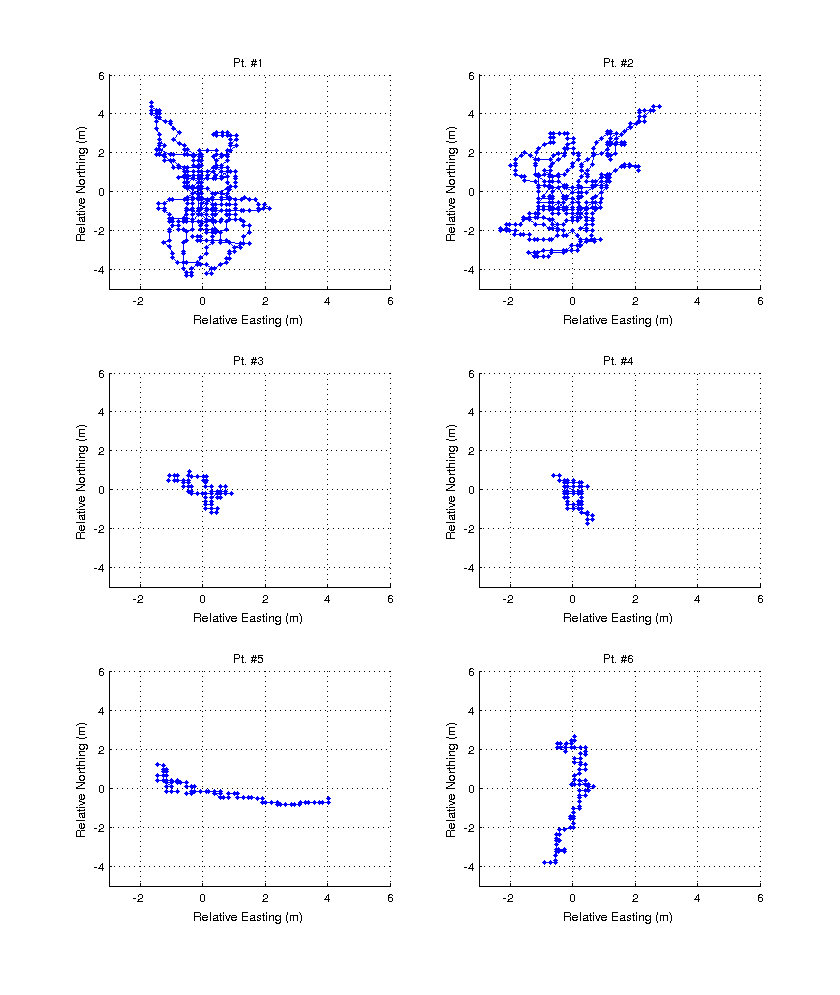
\includegraphics[width=1.1\textwidth]{./img/10min_grid.png}
  \caption{GPS quieto en cada punto del polígono, GPS orientado como se describe en \ref{sec:gps2-procedimiento} y se muestra en \ref{fig:vista_usb.jpg}.}
  \label{fig:10min_grid.png}
\end{figure}

\newpage
En la figura \ref{fig:10m_todos.png} se observan todas las gráficas de la figura \ref{fig:10min_grid.png}, pero superpuestas.

Si el GPS fuese perfecto, entonces todas las muestras coincidirían con el promedio, y estarían ubicadas en el punto \verb+[0,0]+. El círculo negro tiene 2.5m de radio, las muestras que caen fuera de él están a más de 2.5m del valor promedio. En la leyenda se muestra que porcentaje de las muestras caen fuera del círculo.

\begin{figure}[h!]
  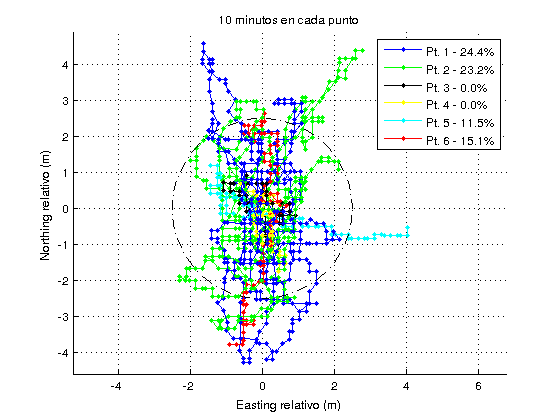
\includegraphics[width=1.1\textwidth]{./img/10m_todos.png}
  \caption{Error respecto al valor medio (Plots de \ref{fig:10min_grid.png} superpuestos). En la leyenda se muestran que porecentaje de muestras que caen a más de 2.5m del promedio.}
  \label{fig:10m_todos.png}
\end{figure}

\newpage
\subsection{Punto fijo - 2 minutos}

Se repitió el experimento tomando solamente 2 minutos de muestras por punto. Se optó por tomar datos durante solamente 2 minutos para agilizar el experimento. Los resultados son similares a los que se obtuvieron con el experimento de 10 minutos.

Se orientó el GPS de 3 maneras distintas, siempre alineando el trípode con uno de los lados de 12m del rectángulo:

\begin{enumerate}
\item USB hacia la calle, LED hacia el estacionamiento, como en la figura \ref{fig:or3.jpg}.
\item USB hacia la rambla, LED hacia el IIE.
\item Como en la figura \ref{fig:or2.jpg}.
\item Nuevamente, USB hacia la calle, LED hacia el estacionamiento, como en la figura \ref{fig:or3.jpg}.
\end{enumerate}

\begin{figure} [h!]
  \centering
  \subfloat[Orientación \#3]{\label{fig:or2.jpg}
  		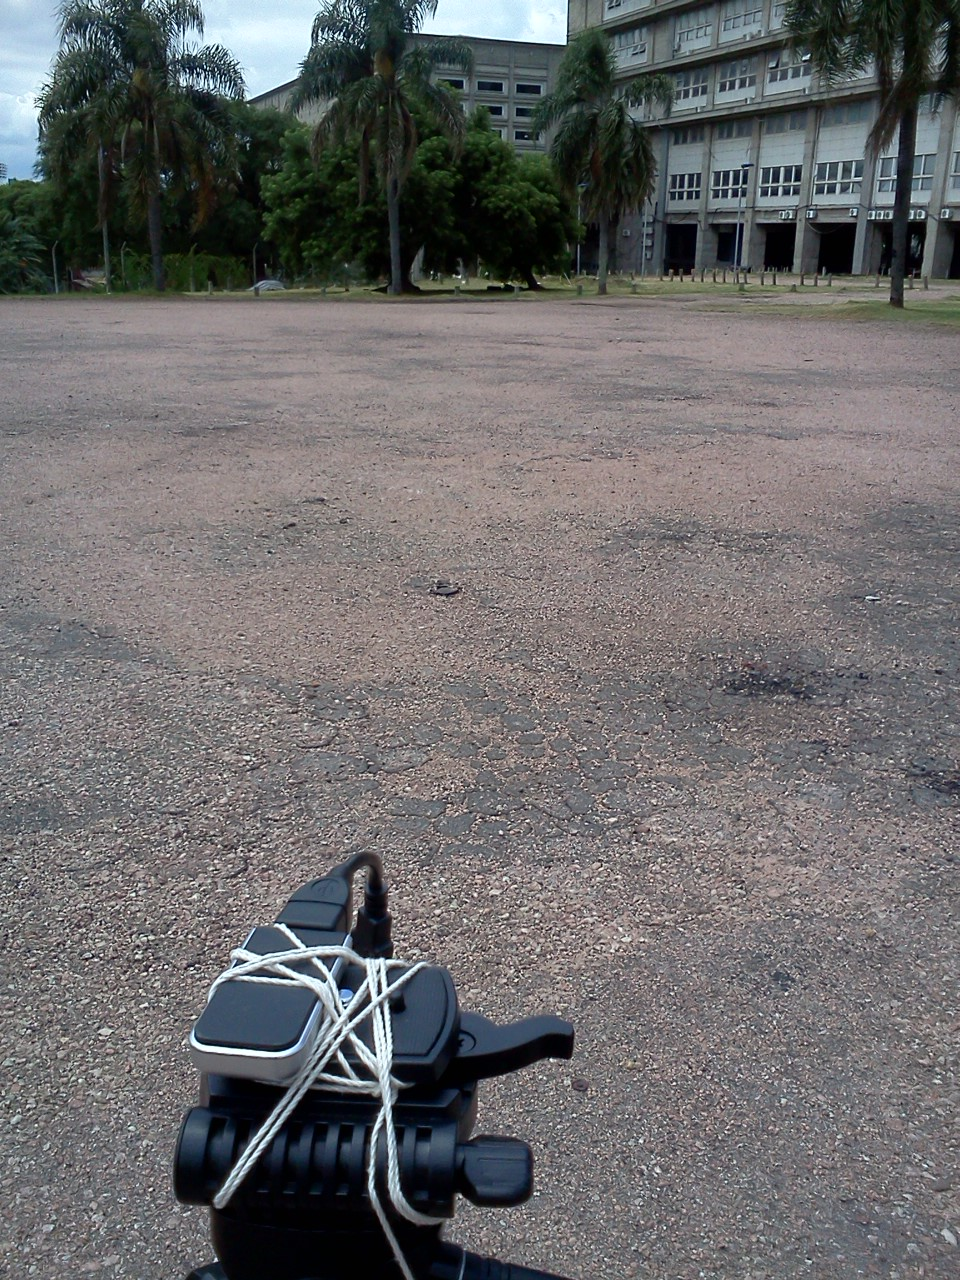
\includegraphics[width=0.45\textwidth]{./img/or2.jpg}}
  \subfloat[Orientación \#4.]{\label{fig:or3.jpg}
  		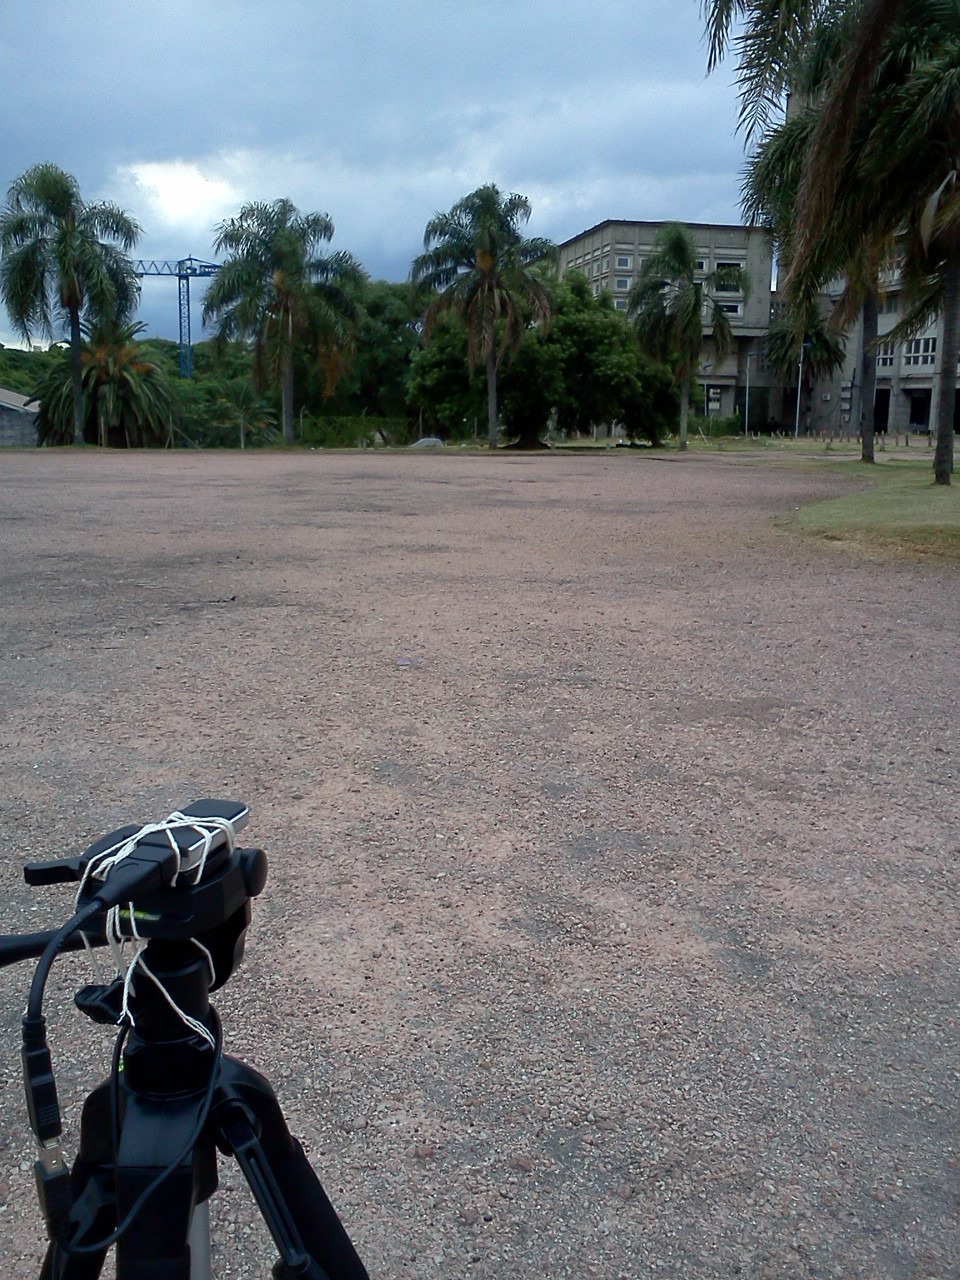
\includegraphics[width=0.45\textwidth]{./img/or3.jpg}}
  \caption{Fotos de algunas de las orientaciones del GPS en las pruebas de 2 minutos por punto.}
  \label{fig:or-2-m}
\end{figure}

Los resultados se observan en las siguientes figuras. Nuevamente, en la leyenda se muestra que \textbf{porcentaje de las muestras a más de 2.5m del valor promedio}.

\newpage
\begin{figure}[h!]
  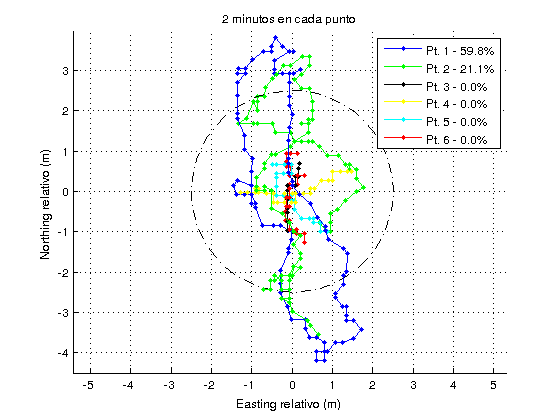
\includegraphics[width=.9\textwidth]{./img/2m_or1_todos.png}
  \caption{Orientación: USB hacia la calle, LED hacia el estacionamiento, como en la figura \ref{fig:or3.jpg}.}
\vspace{-30pt}
  \label{fig:2m_or1_todos.png}
\end{figure}

\begin{figure}[h!]
  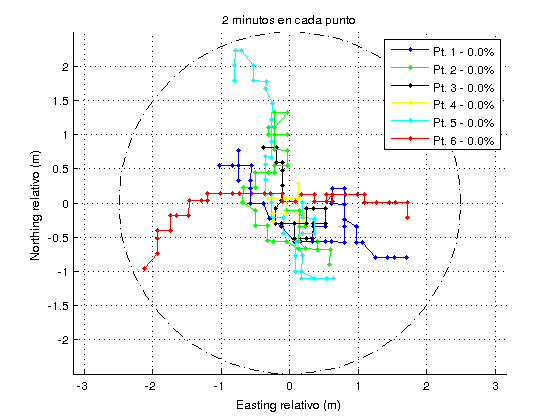
\includegraphics[width=1\textwidth]{./img/2m_or2_todos.png}
  \caption{Orientación: USB hacia la rambla, LED hacia el IIE.}
  \label{fig:2m_or2_todos.png}
\end{figure}

\newpage
\begin{figure}[h!]
  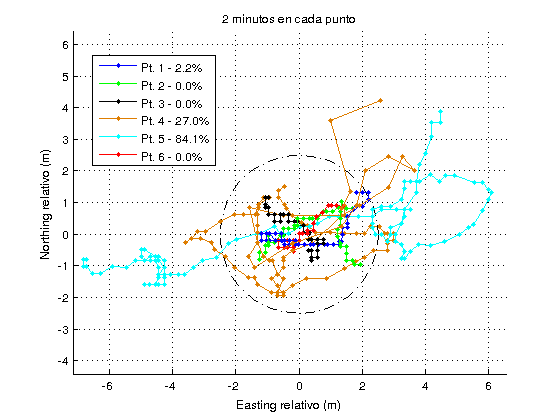
\includegraphics[width=1\textwidth]{./img/or2_todos_cut.png}
  \caption{Orientación: Como en la figura \ref{fig:or2.jpg}.}
\vspace{-30pt}
  \label{fig:or2_todos_cut.png}
\end{figure}

\begin{figure}[h!]
  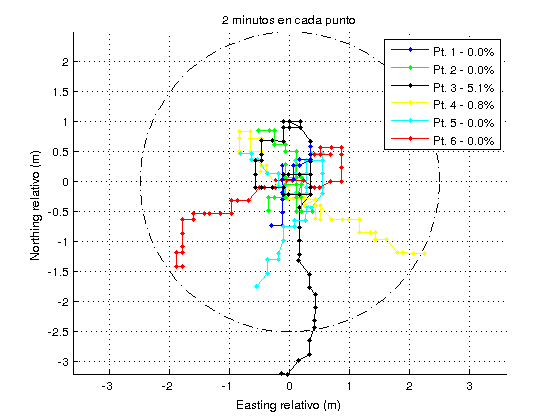
\includegraphics[width=.9\textwidth]{./img/or3_todos.png}
  \caption{Orientación: USB hacia la calle, LED hacia el estacionamiento, como en la figura \ref{fig:or3.jpg}.}
  \label{fig:or3_todos.png}
\end{figure}

\newpage
\subsubsection{Punto fijo: Análisis}
\label{sec:gps2-punto-fijo-conclusiones}

\begin{itemize}
\item Influencia de la cantidad de \textbf{satélites disponbiles}

La teoría dice que con 4 satélites debería alcanzar para obtener un \textit{fix 3D}, es decir, estimar la posición sobre la esfera terrestre, y la distancia (altura) a la misma. Durante el experimento de la figura \ref{fig:or2_todos_cut.png}, en un momento el GPS perdió señal, y el número de satélites disponibles, que usualmente anda por los 9 o 10, pasó a ser 4. Los datos correspondientes se muestran en la figura \ref{fig:or2_todos_sat_mal.png}. El trazo naranja, con un error de hasta 23 metros, corresponde a instantes donde la cantidad de satélites era entre 4 y 5. Luego de volver a 9 o 10 satélites, los datos vuelven a ser más razonables.

\begin{figure}[h!]
  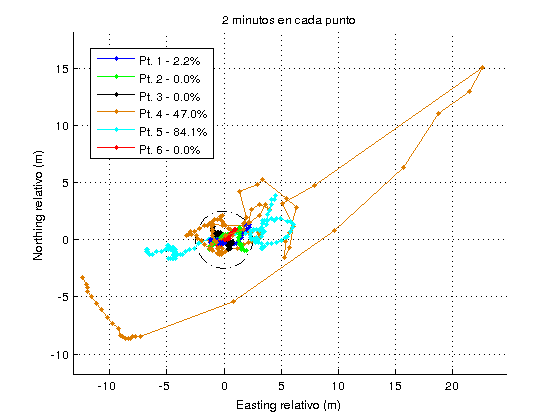
\includegraphics[width=1\textwidth]{./img/or2_todos_sat_mal.png}
  \caption{Datos con solamente 4 satélites. Orientación: Como en la figura \ref{fig:or2.jpg}.}
  \label{fig:or2_todos_sat_mal.png}
\end{figure}

En la figura \ref{fig:or2_todos_cut.png} se observa el mismo log que en \ref{fig:or2_todos_sat_mal.png}, pero luego de haber quitado las muestras correspondientes al período donde se deterioró la señal.

No se pudo encontrar una explicación para la mala calidad de las muestras correspondientes al punto 5 en la figura \ref{fig:or2_todos_cut.png}. La cantidad de satélites disponibles se mantuvo estable en 9 o 10 durante la adquisición de esos datos.
\item Influencia de la \textbf{orientación}:

No parece haber una correlación directa entre resultados y la orientación del GPS, evidencia de esto son las figuras \ref{fig:or3_todos.png} y \ref{fig:2m_or1_todos.png}, que fueron tomadas con la misma orientación.

Resulta  intuitivo suponer que existe, debido a que el GPS tiene una antena adentro. En la sección \ref{sec:gps-orientacion} se estudia un poco más este asunto.
\end{itemize}

\newpage
\subsubsection{Orientación}
\label{sec:gps-orientacion}

Para evaluar si existe una correlación entre la orientación y las medidas del GPS, se hizo el siguiente experimento:
\begin{enumerate}
\item Tomar datos durante 10 minutos con el GPS arriba del trípode, dos patas alineadas con una recta fija.
\item Rotar el trípode 120 grados en sentido horario (visto desde arriba), de manera que otro lado del triángulo que forman las patas del trípode quede alineado con la recta. Tomar datos durante 10 minutos.
\item Rotar y tomar datos nuevamente.
\end{enumerate}

Los resultados del experimento se observan en la figura.

\begin{figure}[h!]
\hspace{-70pt}
  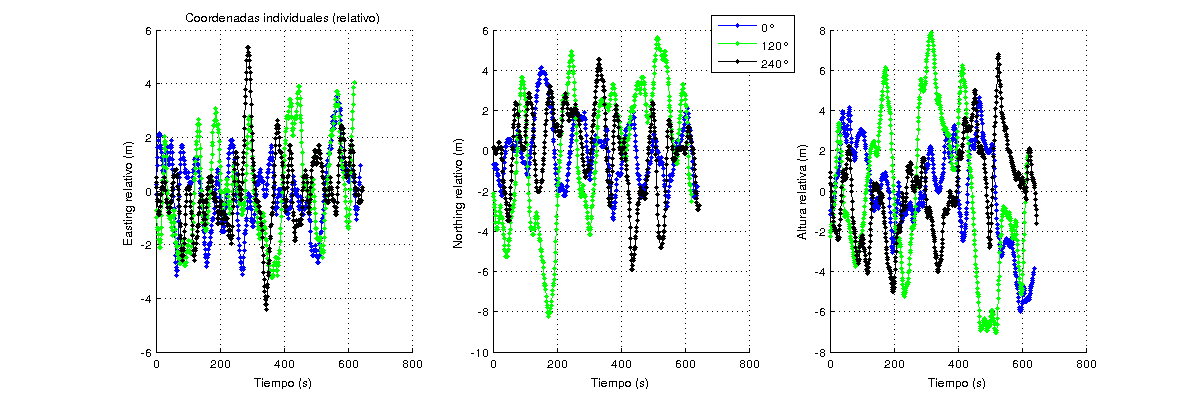
\includegraphics[width=1.4\textwidth]{./img/orientacion_individual.png}
  \caption{Datos rotando el GPS sobre un punto fijo.}
  \label{fig:orientacion_individual.png}
\end{figure}

\subsubsection{Orientación - Conclusiones}
\label{sec:orientacion-conclusiones}

No se encontró una correlación entre la orientación del GPS y el error en las medidas.
El experimento se realizó con cielo abierto, con una buena geometría. Tal vez en situaciones de visibilidad limitada se podría observar una correlación.

Tener visibilidad limitada por obstáculo deteriora la performance del GPS. No es el objetivo de este informe evaluar la performance en ambientes complicados.

\newpage
\subsection{Polígono}
\label{sec:gps2-poligono}

En la figura \ref{fig:10min_pol.png}, en rojo se observa el polígono resultante de unir el promedio de las muestras de 10 minutos tomadas en cada uno de los vértices. En la figura \ref{fig:10m_mapa.png} se dicho polígono, proyectado sobre una foto satelital\footnote{El mapa y las fotos se obtuvieron de \url{http://sig.montevideo.gub.uy/mapas/mapa-principal}} observa lo mismo, pero con promedio de 2 minutos.

\begin{figure}[h!]
  \centering
  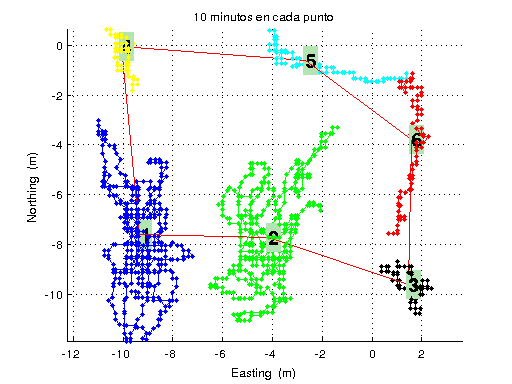
\includegraphics[width=.8\textwidth]{./img/10min_pol.png}
  \caption{Polígono formado por los promedios de 10 minutos.}
  \label{fig:10min_pol.png}
\end{figure}

\begin{figure}[h!]
  \centering
  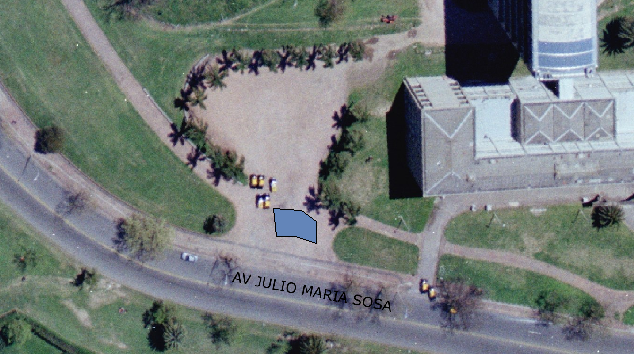
\includegraphics[width=.8\textwidth]{./img/10m_mapa.png}
  \caption{Proyección del polígono formado por los promedios de 10 minutos sobre una foto satelital..}
  \label{fig:10m_mapa.png}
\end{figure}

En las siguiente figuras se observan los polígonos formados por los promedios de varias sequencias de 2 minutos por punto. 

%TODO
% meter fotitos de polígonos
% estimar cada vértice v## como el promedio del log ##, y ver dif entre diag v##-v##' y las medidas con el metro y correjidas con MC
% 
% meter fotito del satelite IMM, con el GPS arriba

\newpage
\section{Conclusión}
\label{sec:conclusion}

Comparando los resultados con secuencias de 2 minutos con el de la secuencia de 10 minutos, se observa que la performance es similar. Se concluye que tomar más de 2 minutos de datos para estimar la posición no reduce el error significativamente, y por lo tanto no vale la pena.

Tomando el promedio de 2 minutos como posición (lat,long, etc) real, se observó que el 75\% de los datos que mide el GPS tienen un error inferior a 2.5m cuando la visibilidad es buena, es decir, cuando el GPS trabaja con 9 o 10 satélites.

Se concluye que es razonable asumir que las medidas del GPS tienen un error de 2.5m.


\end{document}